In the next chapter, this thesis will present the main technologies used. The list of technologies follows the natural order of layers beginning with what have been utilized to construct and train the machine learning models and ending with the technology used for creating the client's application.

\section{Tensorflow}

Tensorflow is a free and open-source software library created originally developed by researchers and engineers working on the Google Brain team within Google's Machine Intelligence Research organization to conduct machine learning and deep neural networks research. It steadily evolved and become one if not the most popular framework to develop machine learning.

Tensorflow is a complex framework containing many layers of abstraction and components to link between different stages of the training and production. It works with other libraries in collaboration in order to facilitate an easier workflow. For our specific problem regarding stock data, Pandas and NumPy will be used along to prepare the data stored in CSV files for the actual model. Lastly, Matplotlib will be used along for generating the initial graphs and plots necessary for comparing different models and methodologies.

NumPy is a library for the Python programming language designed for adding suport to large, multi-dimensional arrays along a large collection of high-level mathematical functions to operate on these arrays. While limiting some of the classic functionalities with array, the library is a staple when it comes to efficient numerical computing in Python.

Pandas is another Python library specialized in data manipulation and data analysis. In particular, it helps tremendously in manipulating numeric tables and time series problems. It is highly customizable and offers seamless integration with CSV files. Its main concept is called DataFrame and represent a 2-dimensional labeled data structure with columns of potentially different types. It provides a large variety of functions built-in such as mean, maximum, minimum or standard deviation, slicing requiring few lines of code to create or normalize data from a source. 

\subsection*{Tensorflow Structure}
Under the hood, Tensorflow works based on the concept of the data flow graph as its computation model. A data flow graph is a model of a program with no conditionals. In a high-level programming language, a code segment with no conditionals—more precisely, with only one entry and exit point—is known as a basic block\cite{levitin2012introduction}. Its main usage is the ease offered in terms of distributing computation across CPUs and GPUs. 

The nodes of the graph are represented by operations, while the edges are tensors. The main Tensorflow entities are: graph, operation, tensor and session. In recent updates, the session is not observed in the foreground, but the other components remain present. As previously mentioned, the graph is build as a set of Operation objects. Each Operation represents a graph node which stems for a unit of computation (addition, multiplication etc.). It takes a tensor as an input and produces a tensor as an output. The tensor is a generalization of vectors or matrices of higher dimensions. They do not represent or hold any particular value produced by an operation in the initial graph. They are used to define the type of value and dimensions acting like a placeholder until the actual execution.

\subsection*{Keras}

Keras is an open-source neural-network library written in Python. It was designed as a high-level interface allowing for fast experimentation of deep neural networks. Tensorflow is supporting its own implementation of Keras fully integrated with its other components.

At its core, Keras offers numerous implementations for commonly used neural-networks building blocks such as layers, objectives, activating functions, loss functions. In addition to standard neural networks, it has support for convolutional and recurrent neural networks. Lastly, utility layers such as dropout, batch normalization or pooling can be easily added.

\section{Spring Framework}

Spring Framework represents an application framework and inversion of control container for the Java platform. While the core features of the framework can be used in any type of Java application, with the extensions there has been a large demand for web-type applications. Since version 5.0, Spring offers official support for the Kotlin language which aims to eliminate the issues of its much known predecessor Java while adding improved features at a much faster pace.

\begin{figure}[H]
\centering
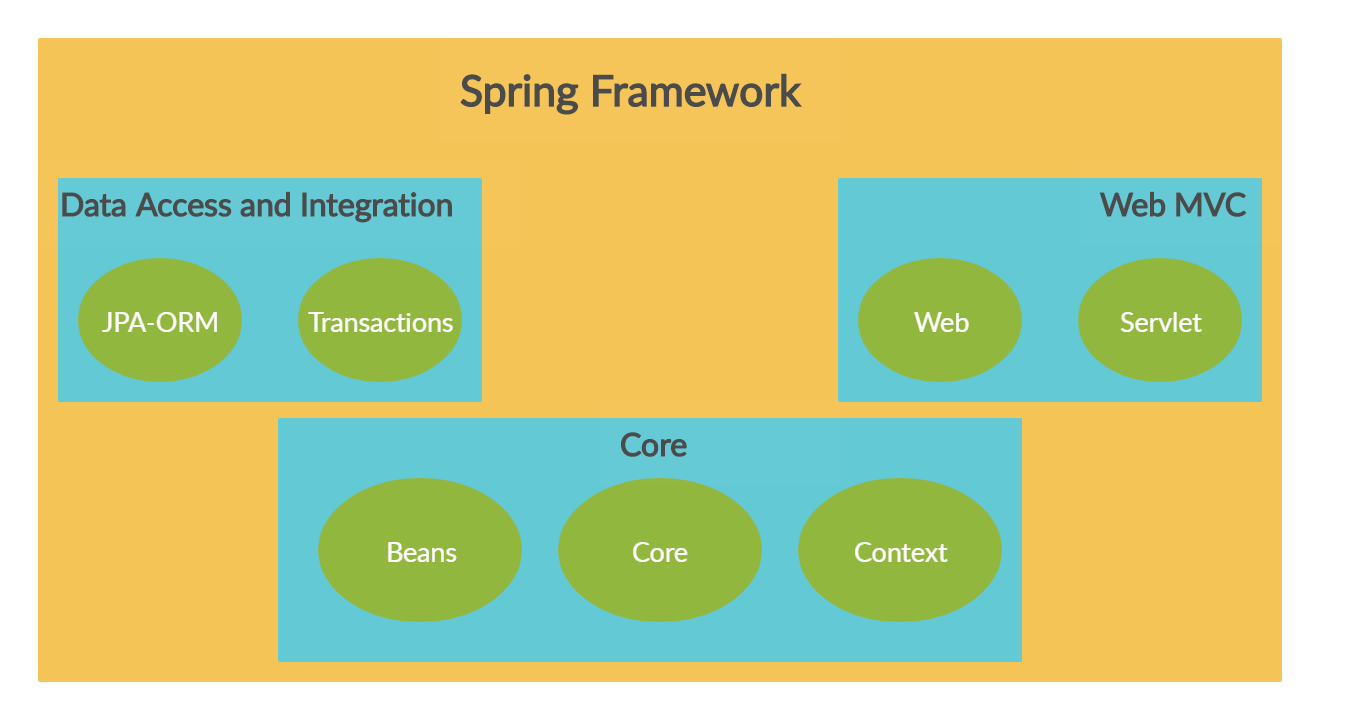
\includegraphics[height=6cm]{images/SpringFramework.png} 
\caption{Spring Framework Components}
\label{fig:springframework}
\end{figure}
\begin{flushright}
Created with: https://creately.com/
\end{flushright}

\subsection*{Spring Inversion of Control}

The spring framework several modules from which the core is definitely one of the most important ones. It offers the implementation of Inversion of Control (IoC) principle and is also known as Dependency Injection (DI). It is a process through which the developer only defines the necessary dependencies between objects through constructor arguments, arguments to a factory method or properties. From that moment, the core container will deal with the actual underlying issues of creating and injecting the instances necessary. As opposed to the general methodology in which the class instance controls the instantiation or location of its dependencies, the process is totally inverse resulting in the name of Inversion of Control.

The basis of the container is represented by two concepts: the beans and the context. A bean is an object that is instantiated, assembled and managed by a Spring IoC container. Besides that, the bean behaves just like the implied behaviour from the developer's implementation. The BeanFactory provides the configuration framework and basic functionality, while the ApplicationContext improves upon the aforementioned class and adds a new variety of operations. Consequently, the ApplicationContext represents the main Spring IoC container and is responsible for the aforementioned tasks. In order to grasp the necessary instructions, configuration metadata is searched and create based on different elements annotated by the developer in its code. The older standard was represented by XML which was steadily replaced by Java annotations and Java code.

In order to facilitate the linking between necessary dependencies, autowiring was introduced as an automated method through which the framework resolve what type of bean to be used and where. To obtain such a behaviour, specific should be given to naming conventions and bean classes such that there would be no conflicts in which two or more beans might be used for the same construction argument etc. The introduction of bean scopes allows to differentiate between different number of instantiations needed for a specific class. The singleton design pattern can be very easily achieved through dependency injection requiring no further boilerplate code prone to errors.

\subsection*{Data Access and Integration}

Spring framework offers an extensive data access module allowing improved usage when communicating with your persistence choice. At its core, there is a transaction management system which provides an abstraction layer such that there will be a consistent programming model despite using different technologies such as Java Transaction Api, Java Database Connectivity or Java Persistence Api. Java Database Connectivity (JDBC) is the barebone application programming interface created by Oracle to define a universal communication standard between the application and various drivers for different database providers. While continuously improved, JDBC has more lately been considered a choice for maintaining only certain types of applications and more modern APIs should be used instead in new applications.

Java Persistence API (JPA) represents a higher level abstraction application programming interface which allows a future key aspect: object-relational mapping. Object-relational mapping allows data conversion between incompatible systems using object-oriented programming languages. In other words, it allows conversion between your domain classes and associated database tables. Spring offers JPA integration through Hibernate which is by far the most object-relational mapping tool for the Java programming language.

JPA offers idiomatic persistence, high performance and reliability. Idiomatic persistence enables the developer to write persistence classes using object orientated classes and linking them to the database structure through various annotations. Its performance stems from the available fetching techniques that can be used in order to load only the relevant data. At its core, JPA creates a small duplicate cached in memory database on which operations are made when executing some commands. Only when a transaction is committed, the changes will be ported over to the real database and will come into effect. In terms of fetching, there are two main fetching strategies: eager and lazy. Eager refers to fetching the entire data in one transaction, while lazy fetching will load some of the data only when needed in some operation. While lazy fetching is preferred, more attention should be made such that you won't access data outside a transaction environment.

In order to promote an intuitive platform for communicating with the layer, Java Persistence Query Language (JPQL) was introduced to break the barrier between SQL and the object-oriented model. JPQL offers a syntax very similar to SQL, but changes the focus on retrieving entities instead of rows or fields. JPA offers extended ORM support with advanced mappings and entity relationships. Advanced mappings offer inheritance support for objects in three different manners: single table, joined table or table per concrete class. In terms of relations, the platform offers the same relations as in the relational database design: one-to-one, one-to-many and many-to-many.

\subsection*{Spring Web Model-View-Controller}

Spring Web MVC framework is the original web framework built on the Servlet API and has been provided since the beginning. It is designed around the concept of a DispatcherServlet which represents the front central controller and provides a shared algorithm for generic request processing while delegating future work to other components. Further, we are going to present only the main components that will be used along for our needs.

Starting with Spring 3.0, the framework allows the usage of the representational state transfer architectural style (REST) in order to create Web services. The framework allows painless declaration of various endpoints based on the HTTP protocol. As a standard transfer format in request, JavaScript Object Notation (JSON) is used and automated binding between JSON and POJO classes is done behind the scenes by some delegate of the DispatcherServlet.

A RESTful system favours a client-server architecture allowing improved performance, scalability or portability. A key concept of REST architectural style is the use of stateless requests by default, but a more detailed explanation will be presented in the next chapter regarding how to deal with statelessness, but maintaining information about what user is requesting the information. In order to filter and log the useful information for each request, the framework a base class GenericFilterBean which allows the custom behaviour to be set for all requests with a specific URI pattern.


\section{Android Software Development Kit}

\subsection*{Android Basics}

Android is the most popular mobile operating system and one of the two major players in the market -alongside iOS. It is based on a modified Linux Kernel and other open source platforms, designed mainly for mobile devices such as smartphones, tablets and Google's version is the one used by almost everyone.

In order to facilitate the software development of third-party apps, Google created and published the Android Software Development Kit (SDK) which allows developers to integrate code mainly at the most upper-level of the system. Under the application layer, there exists a specific hierarchy on top of the Linux kernel, but they aren't concerning the application developers.

Different from many operating systems, an application is Android is almost totally isolated from the rest. Basically, each process in Android has its own Virtual Machine (VM) and each app has its own unique process creating a security sandbox environment. The Android system implements the principle of 'least privilege' which means that each app has access only to the minimal amount of components to work and nothing more. Consequently, each application contains a manifest file which specifies the features, permissions and hardware components which will be used by the application. 

App components represent the building block of any Android application. Each component is considered an entry point to your point, the one accessing being either the user or the system itself. There are four major existing types: activities, services, broadcast receivers and content providers. While each of them has its own lifecycle
and serves a different purpose, activities are widely considered the staple in terms of building blocks. An interesting design aspect is the communication between components. While apps are isolated as mentioned earlier, each component of an application can access an external component of another application through a asynchronous message called 'Intent'. This message is maintained and passed along by the Android System itself in order to respect the previously mentioned isolation points. For this main reason, an Android application hasn't only one entry point as we were used from other systems changing the standard paradigm structure.

\subsection*{Activity Lifecycle}

The activity component is the main process with which you facilitate an independent point of entry in your application. It also provides the layout which will be drawn on the screen by the operating system and usually represents the main interaction point with the user. Each created activity must be added to the manifest file which will contain other options available to extend your activity functionalities.

A core topic in Android is the lifecycle of a specific component, more importantly the lifecycle of an activity. The lifecycle of an activity can be seen as the flow of states through which an activity passes when it is created, paused, destroyed by the system etc. From the development perspective, the Activity class offers a series of callbacks which are called by the system itself when some event happens changing the state of the application. In order to easily present the different states and changes, we are going to use an official simplified schematics from the guidelines.

As we may observe in figure \ref{fig:androidactivitylifecycle}, the activity android lifecycle contains a relatively complicate graph with no more than six core callbacks to which some optional ones can be used in special cases. For an easier presentation, we are going to present them in groups by two similar to a constructor-destructor manner.

Firstly, $onCreate()$ and $onDestroy()$ represent the most 'outer' callbacks called when an activity is created from scratch or destroyed. The create is responsible for basic startup logic usually done once per the lifecycle of the activity such as inflating the initial view or settings listeners for user interactions. Lastly, the method received a parameter called 'bundle' which is maintained by the system to be able to reproduce an activity destroyed while in the background. The $onDestroy()$ method is much less used because many resources are usually released in previous callbacks such as $onPause()$ and $onStop()$. It is called when an activity is finished or a configuration change occur requiring the system to redraw the entire UI. As a rule of thumb, the resources remaining open and becoming unnecessary should be freed in this callback.

\begin{figure}[H]
\centering
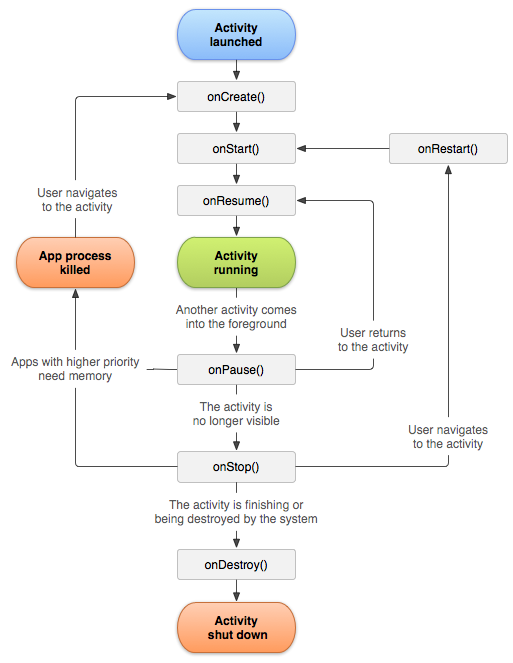
\includegraphics[height=10cm]{images/ActivityLifecycle.png} 
\caption{Android Activity Lifecycle Flow}
\label{fig:androidactivitylifecycle}
\end{figure}
\begin{flushright}
Original picture: https://developer.android.com/guide/components/activities/activity-lifecycle
\end{flushright}

Secondly, $onStart()$ and $onStop()$ represent the callbacks defined at the moment that the activity becomes visible or invisible to the user. The start method is responsible with assuring that any user interface element is totally linked between the activity and user interaction allowing the $onCreate()$ to reduce in general size which has become in many large applications unacceptable to some extent. On the other hand, $onStop()$ is considered more relevant in an importance ranking system because in general an activity should change its intensive behaviour when it is no longer the main focus for the user. It is called when a new activity is launched and will cover over the entire screen or preliminary to $onDestroy()$ when an activity is to be destroyed. The method is responsible to stop or reduce actions which are no longer necessary such as animations, intensive sensor or location tracking and is recommended as the place to use CPU-intensive operations shutdown operations such as database calls.

Lastly, $onResume()$ and $onPause()$ define the interval time frame in which the user can successfully interact with the activity. In general, the $onResume()$ method is only responsible to assure that the elements which may have been disabled in an $onPause()$ callback are fully operating again since we can observe from \ref{fig:androidactivitylifecycle} that there exists the possibility of a small cycle $onResume() -> onPause() -> onResume()$ without going through other lifecycle callbacks. The $onPause()$ method is responsible for releasing resources which aren't necessary while the application is not in the foreground. However, there is an exception for this rule: multi-window mode where your activity might not be in focus, but still visible for the user and still processing (eg. music or video player).

\subsection*{Android Architecture Components}

As we have seen, the Android platform has additional problems to be solved in order to assess the quality of a particular application. As we have presented the activity lifecycle while not mentioning fragments which represent sub-behaviours and sub-interfaces with their separate lifespan, there appeared a difficulty in deciding a suitable architecture for a generic application. Due to these factors, Google has decided to introduce a separate package from the core Android library called Android Jetpack in order to help developers write more high-quality and structured application in an easier manner. In the following paragraphs, we are going to present the 'Android Architecture Components' - a collection of libraries specialized for designing robust and maintainable application with a clean architecture.

The components methodology stem from the standardized structural design pattern decided for Android : Model-View-ViewModel (MVVM). In this manner, there is a clear separation between the data persistance layer (Model) and the user interface layer (View). The ViewModel acts as an intermediary layer between the two and favours event-driven programming exposing Observable objects to the View layer which is responsible to decide how to interpret the new consumed value. In order to achieve this minimum behaviour, three main components were added to facilitate it: Room Persistence Library, ViewModel and LiveData.

Room Persistence Library represents a huge improvement over the default SQLite database providing a supplementary abstraction layer. Even though initially you might get the impression that room allows for basic object-relational mapping, in reality it is strongly discourage due to the limitations and the speed necessary for displaying each frame of an application. It consists of three main set of objects: a database class with annotations for the entities objects, the entities classes which represent each a table in the database and a set of data-access-objects (DAOs) which contain interface with queries specific for the necessary use case. 

LiveData is an observable data holder class. The improvement over a regular observable is the lifecycle awareness integrated in the classs, allowing for ease of use without implementing multiple callbacks to make sure that the lifecycle is respected whether we are talking about an activity, a fragment or a service. In addition to this, LiveData is integrate with Room and has support for Kotlin coroutines allowing for one-way or two-way data binding.

ViewModel class was designed to store and manage UI-related data while maintaining a life-cycle awareness. It was created in order to provide data for the UI even after a configuration change which causes the recreation of the entire user interface. A ViewModel can outlive the activity to which is linked and represents a much improved version of keeping data between changes as opposed to the initial standard bundle.

In addition to all these components, Navigation component and view binding will be incorporated to facilitate moving between different screens. View binding is responsible to create a safe environment for the specific layout used in the screen by compile time checking, while the navigation component allows for the creation and automatization of multiple navigation graphs which will present a clear flow in what actions can the user take to navigate through the application.